
	In chapter \ref{s:background}, we built the space $\MM$ of flat $SU(2)$ connections on a compact connected Riemann surface $\Sigma$ of genus $g\geq 2$, which is a complex projective variety with dimension $3g-3$. Furthermore, $\MM$ is equipped with the Atiyah-Bott symplectic form $\omega$, and in section \ref{s:cs-bundle} we will equip $\MM$ with a prequantum line bundle $(\LL,\nabla)$ over $\MM$ with curvature $2\pi i \omega$.
	
	This system has two notable polarisations one can use to perform a geometric quantization. There is a Kahler polarisation, whose quantization is known to have dimension computed by the \emph{Verlinde formula}, and there is a real polarisation introduced by Weitsman \cite{weitsman_real_1992}. Jeffrey and Weitsman discuss the Bohr-Sommerfeld geometric quantization of $\MM$ with this real polarisation. Bohr-Sommerfeld quantization typically requires a compact symplectic manifold $(M,\omega)$ and line bundle $\LL$, with a real polarization of $M$. A real polarization of $M$ is a map $\pi:M\to B$ onto a manifold of half dimension, such that $\omega|_{\pi^{-1}(b)} =0$ for all $b\in B$. Supposing $\pi:M\to B$ is also a fibration, there will be a finite set of \textit{Bohr-Sommerfeld points} $b_i$ for which $\LL$ restricted to the fibers $L_{b_i}$ of $\pi$ possesses global covariant constant sections. Let $J_\pi$ denote the sheaf of sections of $\LL$ which are covariant constant along the fibres of $\pi$. Then the Bohr-Sommerfeld quantization of a prequantum system $(M,\omega,\LL)$ (for $\pi$) is the vector space
	\begin{equation}
		\mathcal{H} = \bigoplus_{i=0}^{\dim M} H^i(M,J_\pi).
	\end{equation}
	Here we aim to compute the dimension of $\mathcal{H}$. If $B_s$ is the set of all Bohr-Sommerfeld points, and for each $b\in B_s$ $S_b$ is the space of global covariant constant sections of $\LL|_{\pi^{-1}(b)}$, then Sniatycki \cite{sniatycki_cohomology_1977} proves that there is a natural isomorphism:
	\begin{equation}
		\mathcal{H} \cong \bigoplus_{b\in B_s} S_b.
	\end{equation}
	Since each $S_b$ is one dimensional, counting $\dim \mathcal{H}$ boils down to counting the Bohr-Sommerfeld points. 
	
	For the prequantum system on $\MM$ we're considering, the above theorem does not apply because $\MM$ is not a smooth manifold and the polarisation we will describe is not a fibration. Sniatycki's theorem simply provides inspiration for investigating the Bohr-Sommerfeld set in $\MM$, and Jeffrey and Weitsman show that Bohr-Sommerfeld fibres are associated to marked trivalent graphs satisfying the quantum Clebsch-Gordan conditions, and the number of such graphs is called the \emph{Verlinde dimension}, counted by the Verlinde formula \cite[Thm. 8.1]{jeffrey_bohr-sommerfeld_1992}.
	
\section{Prequantum Line Bundle on the Moduli Space}
\label{s:cs-bundle}
	A key part of a prequantum system is the prequantum line bundle $\LL$ with curvature $2\pi i \omega$. Let us build such a bundle over our moduli space $\MM$, following the paper of Ramadas, Singer and Weitsman \cite{ramadas_comments_1989}. Given a connection 1-form $A$ on a 3-manifold $M$, we can define the \textit{Chern-Simons action}:
\begin{equation}
\CS(A) = \frac{k}{2\pi}\int\limits_N A\wedge dA + \frac{2}{3}A\wedge A \wedge A,~ k\in\mathbb{Z}.
\end{equation}
Under a change of gauge $g\cdot A = g^{-1}Ag + g^{-1}dg$, the Chern-Simons action transforms as 
\begin{equation}
\CS(g\cdot A) = \CS(A) - k \int\limits_N d\Tr\left((dg)g^{-1}\wedge A\right) - \frac{k}{3}\int\limits_N \Tr((g^{-1}dg)\wedge (g^{-1}dg)\wedge (g^{-1}dg)).
\label{e:cs-gauge}
\end{equation}\\
The third term on the right side will always be in $2\pi \mathbb{Z}$, and the second term is a total derivative which we can integrate using Stokes theorem over the boundary.

Using this action, we will define a function $\Theta:\cA\times \cG \to \mathbb{C}$. Pick any 3-manifold $N$ for which $\partial N \cong \Sigma$. Given a pair $(A,g) \in \cA\times\cG$, we can always lift it to a choice of $(\tilde{A}, \tilde{g})$ on $N$, since $\pi_1(SU(2)) = \pi_2(SU(2)) = 0$. We define $\Theta$ as
\begin{equation}
\Theta(A,g) = \exp\left[i\CS(\tilde{A}) - i\CS(\tilde{g}\cdot A)\right].
\end{equation}
Equation (\ref{e:cs-gauge}) lets us simplify this;
\begin{align*}
\Theta(A,g) &= \exp(i \CS(\tilde{g}\cdot \tilde{A}) - \CS(\tilde{A}))\\
&= \exp\left[-ik \int\limits_N d\Tr\left((d\tilde{g})\tilde{g}^{-1}\wedge \tilde{A}\right) - 2\pi \kappa\right], \kappa \in \mathbb{Z}\\
&= \exp\left[-ik \int\limits_{\Sigma} \Tr(dg~ g^{-1}\wedge A)\right].
\end{align*}
Note that in the last equality, we use that the lifted pair $(\tilde{A},\tilde{g})$ restricts to $(A,g)$ on $\partial N = \Sigma$ by definition. This computation shows us in particular that $\Theta(A,g)$ is well defined, as it does not depend on our choice of $N$ or the lifting. One can further check that $\Theta$ is a cocycle:
\begin{equation}
\Theta(A,g)\Theta(g\cdot A, h) = \Theta(A,gh).
\end{equation}
Thus we are ready to define $\LL$.
\begin{definition}[Chern-Simons Prequantum Line Bundle]
	\label{d:cs-bundle}
	For $(A,z)\in \cA\times \C$, let $(A,z)\sim (g\cdot A, \Theta(A,g)z)$ under any $g\in \cG$. Then define
	\begin{equation}
	\LL = \cA\times \C / \sim,
	\end{equation}
	which is a complex line bundle on $\MM = \cA/\cG$. Since $\Theta$ is $U(1)$ valued, it is a hermitian line bundle.
\end{definition}
Recall the Atiyah-Bott form, before quotienting out gauge transformations, is the form 
\begin{equation}
\omega(\alpha,\beta) = \frac{i}{2\pi}\int\limits_\Sigma \Tr(\alpha\wedge \beta)
\end{equation}
on $\cA$. We can write it as $\omega = d\sigma$, where $\sigma$ is the one-form
\begin{equation}
\sigma(\alpha) = \frac{i}{4\pi}\int\limits_\Sigma \Tr(A\wedge \alpha).
\end{equation}
Identifying $\mathfrak{u}(1)=i\mathbb{R}$ allows the form $\sigma\in \Omega^1(\cA_0,\C)$ to define a connection one-form on $\cA_0 \times U(1)$. We want to check that $\sigma$ agrees with the pull-back of a unitary connection on $\LL$ with curvature $\omega$, under the map
\begin{equation}
\cA_0 \to \cA_0 \times 1 \hookrightarrow \cA_0 \times U(1) \to \LL.
\end{equation}
The last map comes from quotienting out the action of $\cG$. For $\sigma$ to pass to $\LL$, we want that
\begin{equation}
\sigma_A(\alpha) = \sigma_{A^g}(\alpha) \mod \cG,
\end{equation}
where $\mod \cG$ means the infinitesimal of $\cG$ by adding $d\Theta(\alpha,g)$. We compute
\begin{align*}
\sigma_{A^g}(\alpha) &= \int_\Sigma \Tr\left[(g^{-1}Ag+g^{-1}dg)\wedge \alpha\right]\\
&= \int_\Sigma \Tr\left[g^{-1}Ag \wedge \alpha\right] + \int_\Sigma \Tr(g^{-1}dg \wedge \alpha)\\
&= \sigma_{A^g}(\alpha) + d\Theta(\alpha,g).
\end{align*}
Therefore, the connection $\sigma$ passes to a connection on $\LL$, with curvature $\omega$. 

There is another construction of a prequantum line bundle for $\MM$, the \textit{determinant line bundle} $\LL_D$ of Quillen \cite{quillen_determinants_1985}. Ramadas, Singer and Weitsman prove that
\begin{theorem}
	\label{t:cs=det}
	The line bundle $\LL$ defined above is isomorphic to the determinant bundle $\LL_D$ as a hermitian line bundle with connection on $\MM$.
\end{theorem}
\begin{proof}
	Ramadas, Singer, Weitsman \cite[Theorem 2]{ramadas_comments_1989}
\end{proof}	
	
	
\section{Polarisation of the Moduli Space}	
	As before, let $\Sigma$ be a compact Riemann surface and $\MM$ the moduli space of flat $G=SU(2)$ connections on $\Sigma$. Following Jeffrey and Weitsman \cite{jeffrey_bohr-sommerfeld_1992}, we describe an action of $T^{3g-3}$ on $\MM$. Let $C$ be a closed oriented curve in $\Sigma$ and pick a basepoint $y\in C$. We can define a function $\tilde{f}_C:\cA \to \mathbb{R}$ by 
	\begin{equation}
		\tilde{f}_C(A) = \frac{1}{2}\text{hol}_C(A),
	\end{equation}
	where hol$_C(A)$ means the holonomy of $A$ around $C$ from $y$ to $y$. Since the holonomy is $\cG$ invariant, this passes to $f_C:\MM \to \mathbb{R}$. $\Sigma$ admits a decomposition into \textit{trinions} or \textit{pairs of pants}, which are copies of a disc with two holes:
	\begin{equation}
		D = \{z \in \mathbb{C}~|~ |z|\leq 2 \} - \{z~|~|z-1|<1/2\}\cup \{z~|~ |z+1| < 1/2\},
	\end{equation}
	with marked points on the boundary of $D$. 

	\begin{figure}[h]
		\centering
		\label{fig:torusdecomp}
		\subfloat[][One decomposition for surfaces of genus $g\geq 2$.]{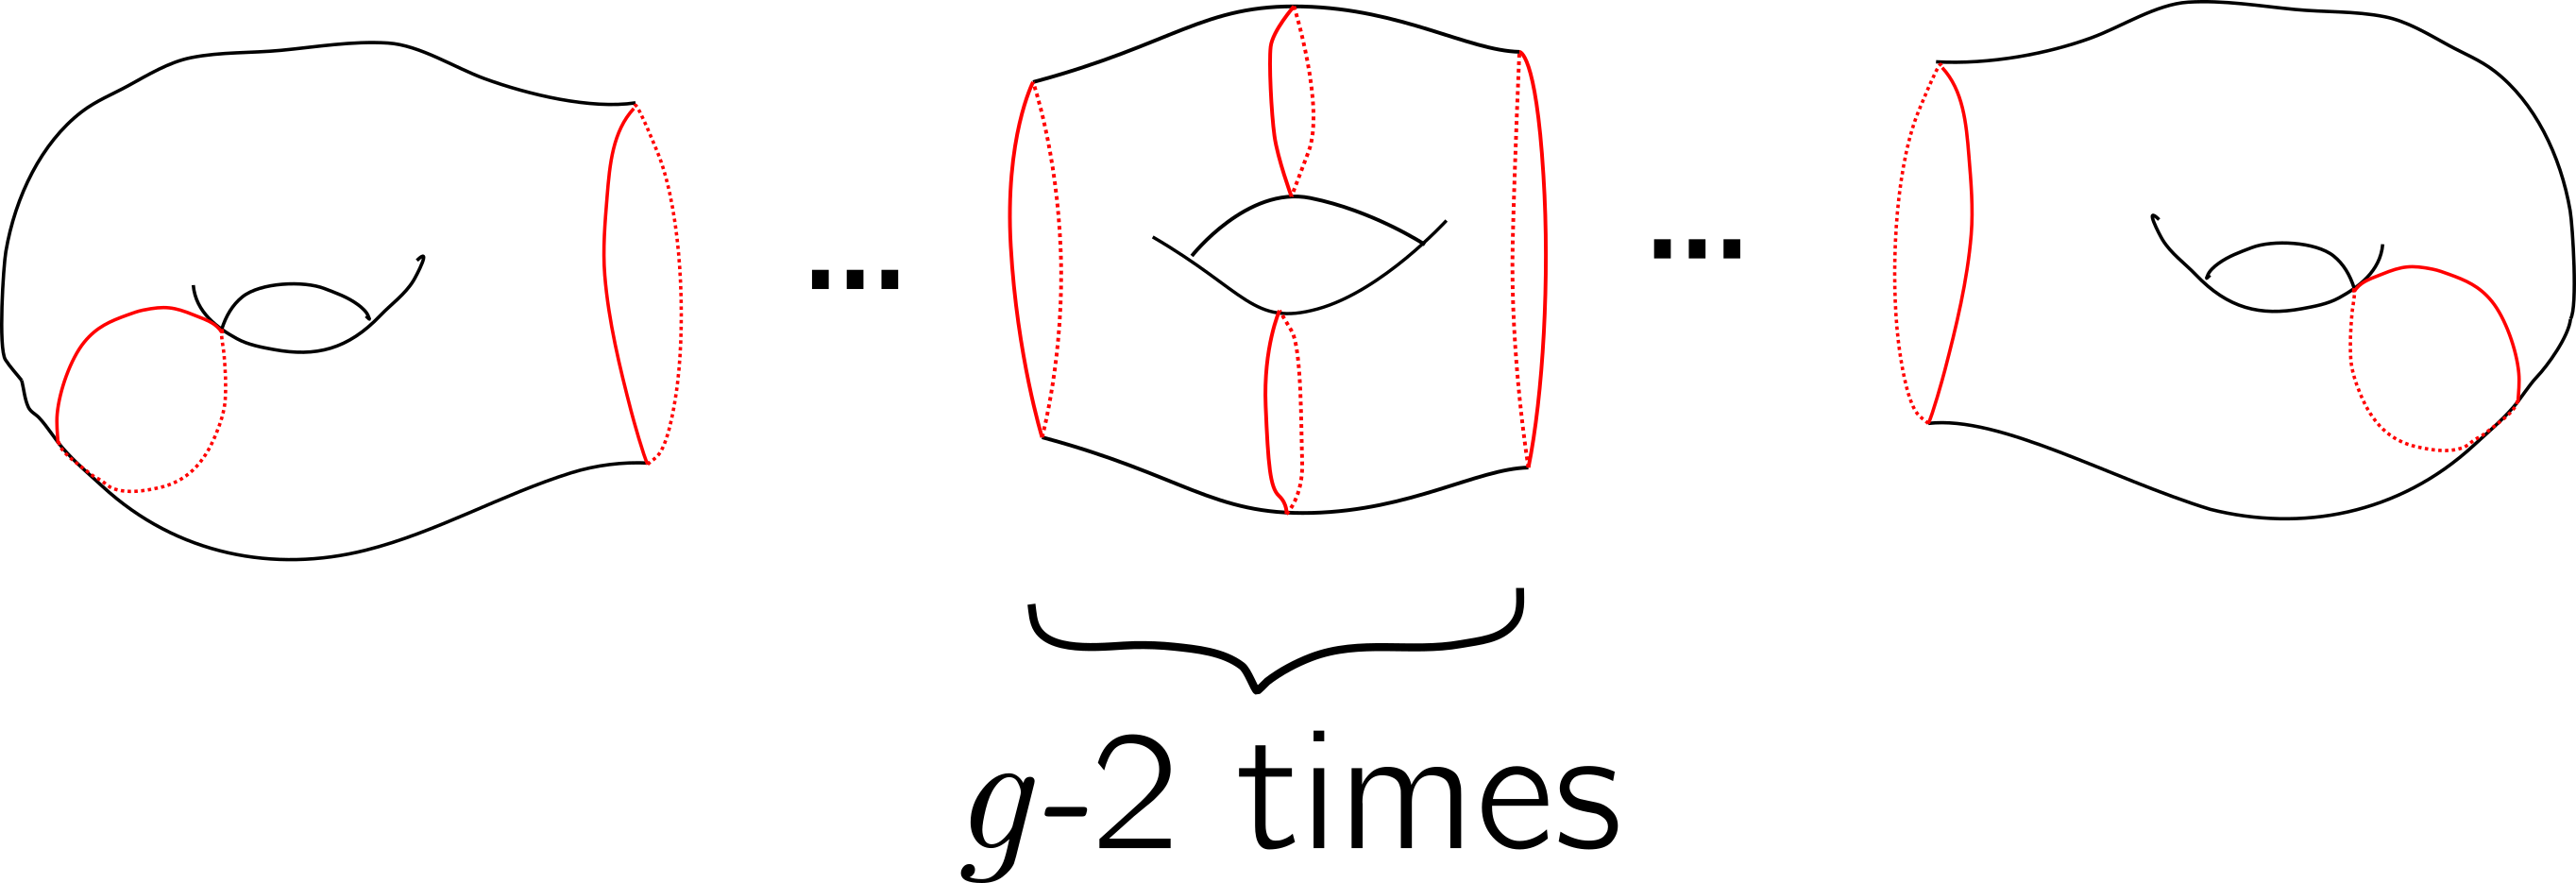
\includegraphics[width=0.4\linewidth]{genusg.png}\label{fig:genusg}}
		\hspace{0.1\linewidth}
		\subfloat[][A different decomposition for $g=2$.]{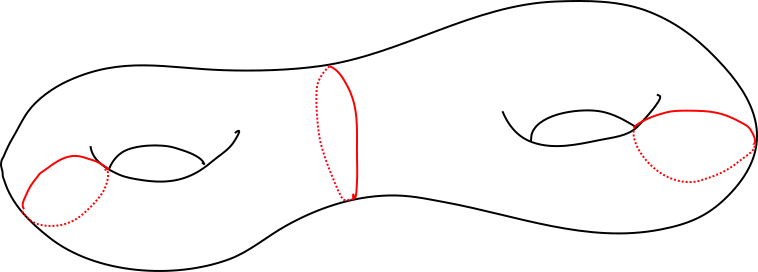
\includegraphics[width=0.35\linewidth]{g2sym_nolabels.png}\label{fig:genus2}}
		\caption{Decomposition of a surface $\Sigma$ into $2g-2$ trinions. }
	\end{figure}

	Suppose we are given such a decomposition of $\Sigma$ into $2g-2$ trinions $D_\gamma$, $\gamma\in\{1,2,...,2g-2\}$, joined along their boundaries and with the marked points on the boundaries coinciding for any trinions with non-trivial intersection. Then the boundary circles of $D_\gamma$ give a collection $C_i$, $i\in\{1,2,...,3g-3\}$ of closed oriented curves in $\Sigma$ for which we get corresponding functions $f_i = f_{C_i}:\MM \to \mathbb{R}$ using the above definition. Since these functions are the trace of $SU(2)$ matrices, they can be described by cosine of angles $\theta_i$,
	\begin{equation}
		\theta_i(A) = \cos^{-1}(f_i(A)),
	\end{equation}
	where $\theta_i$ is taken to lie in $[0,\pi]$. This defines a map $\theta = (\theta_1,...,\theta_{3g-3}):\MM \to \mathbb{R}^{3g-3}$. These $\theta_i$ are smooth on $U_i := \theta_i^{-1}(0,\pi) \subset \MM$, which is open and dense. Thus, the Hamiltonian flows of each $\theta_i$ are defined on $\MM^{s} = \bigcap_{i=1}^{3g-3} U_i \subset \MM$. These Hamiltonian flows are periodic with constant period, which means they induce a torus action on $\MM^{s}$. Explicitly, if we let $X_i$ denote the Hamiltonian vector field of $\theta_i$, defined by
	\begin{equation}
		\iota_{X_i}\omega = d\theta_i,
	\end{equation}
	and let $e^{tX_i}$ be the corresponding vector field flow, then the action is given by $g = (\alpha_1,...,\alpha_{3g-3}) \in T^{3g-3}$ acts by
	\begin{equation}
		A \to e^{\alpha_1 X_1 + ... + \alpha_{3g-3}X_{3g-3}}A.
	\end{equation}
	 The Lie algebra of $T^{3g-3}$ is $
	\mathbb{R}^{3g-3}$ and we interpret $\theta(A)$ as being dual by $\langle \theta, X \rangle = \sum \theta_i X_i$. Then
	\begin{equation}
		d\left(\langle \theta(A),X\rangle\right) = d\sum\theta_i X_i = \sum X_i d\theta_i = \iota_{X}\omega,
	\end{equation}
	which means $\theta$ is the moment map for the torus action. These functions $f_i$ also give us a real polarization of $\MM$. Let $B \subset \mathbb{R}^{3g-3}$ be the image of the $f_i$,
	\begin{equation}
		B = \{(f_i(E),...,f_{3g-3}(E))~|~ E \in \MM\},
		\label{e:B-def}
	\end{equation}
	then the fibers of the map $\pi = (f_1,...,f_{3g-3})$ foliate the smooth locus of $\MM$, and the generic fibre is a Lagrangian subvariety. 
	
	Alternatively, one can describe the polarization using the picture of connections as representations of the fundamental group $\pi_1(\Sigma)$. First, a preliminary result. Let $T\subset SU(2)$ be a maximal torus.
	\begin{definition}
		\label{d:atd-conn}
		A connection $A$ on $\Sigma^g$ is said to be \emph{adapted to a trinion decomposition} (a.t.d.) if there is a tubular neighbourhood $V_i \cong (-1,1)\times S^1$ of each boundary circle $C_i$ in the decomposition, such that in co-ordinates $(s,\theta)$ for $V_i$,
		\begin{equation}
			A|_{V_i} = X_i d\theta, 
		\end{equation}
		where $X_i$ is a constant element in $\mathfrak{t} = \text{Lie}(T)$.
	\end{definition}
	\begin{theorem}
		\label{t:atd-thm}
		For all $y\in \pi^{-1}(b)$, there exists an adapted to trinion decomposition connection $A$ in the gauge equivalence class $y \mod \cG$.
	\end{theorem}
	\begin{proof}
	First, any boundary circle $C$ in a trinion decomposition has tubular neighbourhood $V\cong C\times [-1,1]$ and co-ordinates $(s,\theta)$ in which the connection $y$ takes the form:
	\begin{equation}
		y = R(s,\theta)d\theta + S(s,\theta)ds,
	\end{equation}
	for some $R,S \in C^\infty(\Sigma, \mathfrak{su}(2))$. Suppose we have a gauge transformation $h(s,\theta)$ with $\partial_s h(s,\theta)=0$, $h(0,0)=\mathds{1}$ and
	\begin{equation}
		\label{e:atd-pde1}
		\frac{\partial h}{\partial \theta} - Rh = 0.
	\end{equation}
	Then the $\theta$ component of $h\cdot y$ will be 
	\begin{equation}
		h^{-1}\left(\frac{\partial h}{\partial \theta} - Rh\right) = 0.
	\end{equation}
	Such an $h$ must exist as Equation (\ref{e:atd-pde1}) is four linear first order ODEs for the components of the matrix $h$. One must only check that this solution will be an $SU(2)$ matrix for all $s$ as required. At $\theta=0$, $h = \mathds{1}$, and the derivative is $-R(0,0) \in \mathfrak{su}(2)$; therefore the solution starts in $SU(2)$ and its derivative for all time is an $\mathfrak{su}(2)$ matrix, so the solution remains in $SU(2)$. Notice that $h(0) \neq h(2\pi)$ so this gauge transformation exists on $[0,2\pi]\times[-1,1]$ but it does not pass to $V$.
	
	Now let $H=h(0,2\pi)$ and let $X \in \mathfrak{t}$ be the element such that $\exp(2\pi X) = H^{-1}$ and define $f(s,\theta) = \exp(\theta X)$. Then $\partial_s f = 0$, $\partial_\theta f = Xf$ and 
	\begin{equation}
		f\cdot h \cdot y = f^{-1}Xfd\theta + f^{-1}h^{-1}\left(\frac{\partial h}{\partial \theta} - Rh\right)f + S(s,\theta)ds = Xd\theta + S(s,\theta)ds.
	\end{equation}
	Furthermore $fh(0,0) = \mathds{1}$ and $fh(0,2\pi) = H^{-1}H = \mathds{1}$ so the gauge transformation $fh$ satisfies the periodic boundary condition and is well defined on $V$. Thus it remains to find a gauge transformation sending the $ds$ component to zero. Such a transformation must satisfy 
	\begin{equation}
		\label{e:atd-pde2}
		\frac{\partial k}{\partial s} - Sk = 0,
	\end{equation} 
	with $k(-1,\theta) = \mathds{1}$ and $\partial_\theta k = 0$. As before Equation (\ref{e:atd-pde2}) is four first order ODEs with a unique solution, and the same argument as before shows $k$ will be in $SU(2)$. The $s$ co-ordinate has no periodic boundary condition, so $k$ immediately passes to $V$, and the composition $g = kfh$ gives us our gauge transformation on $V$ putting $y$ in the desired form.
	
	Repeating this process for each boundary circle $C_i$ in our decomposition gives a set of local gauge transformations $g_i$ on each $V_i$. Complete $V_i$ to a cover $\{U_i\}$ of $\Sigma$ and let $g_i = \mathds{1}$ on the additional sets added. Within each $V_i$, pick a smaller tubular neighbourhood $W_i$, and let $\{\phi_i\}$ be a partition of unity for $\{U_i\}$ with $\phi_i = 1$ on $W_i$. Define the global gauge transformation $g = \sum g_i \phi_i$. Then for all $i$, $(g\cdot y)|_{W_i} = X_i d\theta_i$ and so $g\cdot y$ is an a.t.d. representative for $y \mod \cG$.
	\end{proof}
	
	This lets us define subgroups of $G=SU(2)$, which correspond to stabilizers of flat connections. Suppose $A$ is an a.t.d connection. Then the stabilizer of $A|_{C_i}$ in $\cG(C_i) = \Hom(C_i, G)$ consists of constant maps, and can thus be identified with a subgroup $H_i$ in $G$. If $\theta_i(A) \in \{0,\pi\}$, then $\text{hol}_{C_i}(A) = \pm\text{Id}$ and so $H_i = G$. Otherwise, $H_i = T$. 
	
	We can describe the fibre $\pi^{-1}(b)$ using these subgroups. Suppose $A$ is a.t.d. and $[A] \in \pi^{-1}(b)$. Let $\tau_i \in H_i$ for each circle $C_i$, $i\in (1,2,...,3g-3)$. Then define the map
	\begin{equation}
		\label{e:psiA}
		\psi_A : \prod_{i=1}^{3g-3} \to \pi^{-1}(b)
	\end{equation}
	as follows. Denote the trinions composing $\Sigma$ as $D_{\gamma}$, $\gamma\in{1,2,...,2g-2}$. For any circle $C_i$, let $D_{\gamma(i)}$, $D_{\gamma'(i)}$ be the trinions on either side. For $\tau=(\tau_1,\tau_2,...,\tau_{3g-3})$, choose a collection of maps $\zeta_\gamma : D_\gamma \to g$ such that for every $C_i$, $\zeta_{\gamma(i)}$ and $\zeta_{\gamma'(i)}$ are constant on a tubular neighbourhood of $C_i$, and such that
	\begin{equation}
		\zeta_{\gamma(i)}|_{C_i} = \tau_i \zeta_{\gamma'(i)}|_{C_i}.
	\end{equation}
	Here, adopt the convention that the orientation of the tubular neighbourhood is $v\wedge w$, where $w$ is tangent to the oriented circle $C_i$ and $v$ is transverse to $c_i$ and pointing \textit{into} $D_{\gamma(i)}$, thus away from $D_{\gamma'(i)}$.
	
	Now we define a connection $A_\tau$ on $\Sigma$ by defining $A_\tau$ on each trinion: $A_\tau|_{D_\gamma} := \zeta_\gamma \circlearrowright A|_{D_\gamma}$. Finally define $\psi_A(\tau) = [A_\tau]$. Next we ask, for $\tau,\tau' \in \prod_{i=1}^{3g-3} H_i$, when are $A_\tau$ and $A_{\tau'}$ gauge equivalent? 
	
	Let $J_\gamma$ be the stabilizer of $A|_{D_\gamma}$ under $\cG|_{D_\gamma} = \Hom(D_\gamma,G)$. Since $A$ is a.t.d., this also consists of constant maps. $J_\gamma = Z(G) = \{\pm \text{Id}\}$ if the holonomy is an irreducible representation of $SU(2)$, and otherwise $J_\gamma =T$ (resp $G$) if the holonomy reduces to $T$ (resp $Z(G)$).  
	
	Jeffrey and Weitsman prove the following lemma and theorem:
	\begin{lemma}
		If $\tau,\tau'$ are in $\prod_{i=1}^{3g-3} H_i$, then $[A_\tau] = [A_{\tau'}]$ if and only if there is a set of gauge transformations $\Phi_\gamma:D_\gamma \to G$ such that:
		\begin{enumerate}
			\item $\Phi_\gamma \in J_\gamma$ for all $\gamma$.
			\item For each boundary circle $C_i$, we have
			$$
				\Phi_{\gamma'(i)}|_{C_i} \tau_i = \tau_i' \Phi_{\gamma(i)}|_{C_i}.
			$$
		\end{enumerate}
	\end{lemma} 
	\begin{theorem}
		The map $\psi_A:\prod_i H_i \to \pi^{-1}(b)$ is surjective and the group $\prod_\gamma J_\gamma$ has a natural action on $\prod_i H_i$ so that
		\begin{equation}
			\pi^{-1}(b) = \left(\prod_i H_i\right)/\left(\prod_\gamma J_\gamma\right).
		\end{equation}
	\end{theorem}
	\begin{proof}
		Jeffrey and Weitsman \cite{jeffrey_bohr-sommerfeld_1992}, lemma 2.4 and theorem 2.5 respectively.
	\end{proof}

\section{Moduli of Connections on a Trinion}
	In order to build the moduli space $\MM$ by gluing together connections defined along a trinion decomposition, one must first understand the possible connections on one trinion $D$, denoted $\MM(D)$. As in section \ref{s:moduli-as-reps}, $\MM(D)$ can be described by the set $\Hom(\pi_1(D),G)/G$. For a trinion, 
	\begin{equation}
		\pi_1(D) = \left\{
		[C_1], [C_2], [C_3] ~|~ [C_1][C_2][C_3]  =1
		\right\},
	\end{equation}
	where $C_i$ are the three boundary curves of the trinion. We can again define the holonomy angle functions, first letting $\tilde{\theta_i}:\Hom(\pi_1(D),G) \to [0,\pi]$ be
	\begin{equation}
		\label{e:thetacoords}
		\tilde{\theta_i}(\rho) = \cos^{-1}\left(\frac{1}{2}\Tr(\rho[C_i])\right),
	\end{equation}
	and these maps will descend under the quotient by $G$ to maps $\theta_i:\MM(D)\to [0,\pi]$. Then Jeffrey and Weitsman prove \cite[Proposition 3.1]{jeffrey_bohr-sommerfeld_1992}:
	\begin{theorem}[]
		The map $\theta = (\theta_1, \theta_2, \theta_3):\MM(D)\to[0,\pi]^3$ sends $\MM(D)$ bijectively to the set satifying the inequalities
		\begin{equation}
			|\theta_1 - \theta_2| \leq \theta_3 \leq \min(\theta_1 + \theta_2, 2\pi - (\theta_1 + \theta_2)).
			\label{e:trinion-ineqs}
		\end{equation}
		These inequalities define a convex polytope in $\mathbb{R}^3$.
	\end{theorem}

	\begin{figure}[h]
	\centering
	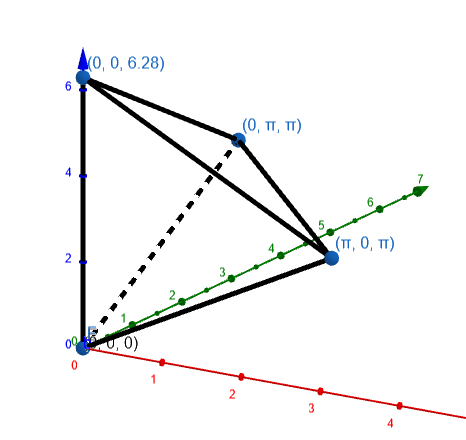
\includegraphics[width=0.5\linewidth]{polytope.png}\label{fig:polytope}
	\caption{The polytope defined by the inequalities (\ref{e:trinion-ineqs}).}
	\end{figure}

	Using this result, and the gluing process described in the last section, the image of $\MM$ under the holonomy angles $\theta_1,...,\theta_{3g-3}$ are the values satisfying the inequalities (\ref{e:trinion-ineqs}) on every trinion. Applying a theorem of Guillemin and Steinberg \cite{guillemin_gelfand-cetlin_1983} to this case, one obtains:
	\begin{theorem}
		\label{t:torusfibres}
		Suppose $x\in \pi(\MM) \subset B$ (defined in eqn. \ref{e:B-def}) Then
		\begin{itemize}
			\item The Hamiltonian vector fields corresponding to the functions $\theta_i$ are linearly independent on the fibre $\pi^{-1}(x)$, if and only if $x$ is a point where all the inequalities (\ref{e:trinion-ineqs}) are strict.
			\item In general, the number of linearly independent Hamiltonian vector fields on the fibre $\pi^{-1}(x)$ is equal to $3g-3-s$, where $s$ is the number of independent linear equations out of the following satisfied by $\theta(x)$:
				\begin{align}
					\label{e:theta-ineqs1}
					\theta_{i_{\sigma(1)}(\gamma)}(x) + \theta_{i_{\sigma(2)}(\gamma)}(x)-\theta_{i{_\sigma(3)}(\gamma)}(x)&=0,\\
					\theta_{i_1(\gamma)}(x) + \theta_{i_2(\gamma)}(x) + \theta_{i_3(\gamma)}(x) = 2\pi.
					\label{e:theta-ineqs2}
				\end{align}
			where $\sigma:{1,2,3}\to{1,2,3}$ is any cyclic permutation. These inequalities correspond to $(\ref{e:trinion-ineqs})$.
		\end{itemize}
	\end{theorem}
	Furthermore
	\begin{lemma}
		Let $x\in \MM(D)$ and let $\theta(x)$ be the holonomy angles of $x$ around the three boundary curves of $D$. Then $x$ corresponds to a conjugacy class of reducible representations of $\pi_1(D)$ if and only if at least one of the equations (\ref{e:theta-ineqs1}),(\ref{e:theta-ineqs2}) above is satisfied.
	\end{lemma}
	Motivated by this lemma, define \emph{interior triples} in $[0,\pi]^3$ to be those for which none of the equations is satisfied, i.e those on the interior of the convex polytope. These triples correspond to points in $\MM(D)$ which are conjugacy classes of irreducible representations of $\pi_1(D)$. Theorem \ref{t:torusfibres} tells us that the fibre $\pi^{-1}(x)$ is a torus of dimension $3g-3$ if and only if $\theta(x)$ is an interior triple.
	\begin{theorem}
		Let $x\in B$ and let $A$ be a flat a.t.d. connection whose gauge equivalence class is in $\pi^{-1}(x)$. Further, assume that on every trinion the holonomy angles of $x$ is an interior triple. Then the fibre $\pi^{-1}(x)$ is identified with $T^{3g-3}/(\mathbb{Z}_2)^{2g-2}$ under the map $\psi_A$ defined in eqn. (\ref{e:psiA}).
	\end{theorem}
	Thus, the fibres corresponding to interior triples, which are the generic fibres, are tori of dimension $3g-3$. 
	
	\section{Counting Bohr-Sommerfeld Points}
	With this real polarization of the moduli space, Jeffrey and Weitsman proceed to count the number of Bohr-Sommerfeld points. In this section we will summarize the results that we want to use going forward.
	
	\begin{definition}
		Let $(\MM,\omega)$ be a symplectic manifold with prequantum line bundle $\LL$ and polarisation $\pi:\MM\to B$. A point $b\in B$ is called a \emph{Bohr-Sommerfeld} point if $\LL|_{\pi^{-1}(b)}$ possess a one-dimensional family of global covariant constant sections.
	\end{definition}
	The quantization of a prequantum system is $\mathcal{H} = \bigoplus_{i=1}^{\dim M} H^i(M, \mathcal{J}_\pi)$, where $\mathcal{J}_\pi$ is the sheaf of sections of $\LL$ covariant constant along the fibres of $\pi$. Sniatycki's theorem \cite{sniatycki_cohomology_1977} proves that when the polarisation of a symplectic manifold is a fibration, the dimension of $\mathcal{H}$ is given by the number of Bohr-Sommerfeld points. Although this result does not apply here, it still provides motivation for counting the Bohr-Sommerfeld points.
	
	One characterization of the Bohr-Sommerfeld points is as the set of points $b$ whose fibres $L_b = \pi^{-1}(b)$ satisfy the property that if $\pi_1(L_b)$ is generated by a set of loops, then the holonomies of the prequantum connection aronud those loops are all equal to $\mathds{1}$. A basis of loops can be obtained in terms of a basis of a lattice of functions $\Lambda$ on $B$, called the \emph{period lattice}. 
	\begin{definition}
		For $\alpha \in T_x^\ast B$, let $v_\alpha$ denote the vertical vector field along the fibre $L_x$ defined by $\pi^\ast(\alpha)$. Let $f_\alpha$ denote the diffeomorphism of the fibre $L_x$ induced by flowing along $v_\alpha$ for time 1.
		
		Then the \emph{period lattice} in $T_x^\ast B$ is the set of $\alpha$ whose corresponding $f_\alpha$ is trivial.
	\end{definition}
	This is a lattice of dimension $m$, and one may show that there is a neighbourhood $U$ of any point $x\in B$ on which there exist functions $\{H_i\}$ forming a lattice $\Lambda$ under addition, such that the period lattice for all $x\in U$ is given by $\{(dH_i)_{x'}\}$ \cite{duistermaat_global_1980}. This lattice will also be referred to as the \emph{period lattice}.
		
	Let $\{\tilde{\mu}_i\}\in C^\infty(B,\mathbb{R})$ be a basis of the period lattice, and define $\mu_i = \tilde{\mu}_i\circ \pi \in C^\infty(\MM,\mathbb{R})$. Then the Hamiltonian flows of the $\mu_i$ have period 1, and the fundamental group $\pi_1(L_x)$ is generated by the loops $\gamma_i$ which are the period 1 trajectories of the Hamiltonian flows of $\mu_i$. The functions $(\mu_1,...,\mu_m)$ define a moment map for a torus $(S^1)^m$ action on on $\MM$, preserving the Lagrangian fibration \cite[\S4]{jeffrey_bohr-sommerfeld_1992}. These functions correspond to a set of \emph{action variables} to pair with our $\theta_i$ angle variables on $\MM$. The period lattice is important, as Jeffrey and Weitsman show that the Bohr-Sommerfeld points correspond to integer values of a set of functions generating the period lattice \cite[\S5]{jeffrey_bohr-sommerfeld_1992}. 
	
	For $\Sigma$ a connected compact Riemann surface of genus $g$, fix a trinion decomposition $\{D_\gamma\}$, and label the boundary loops of $D_\gamma$ as $C_{i_1(\gamma)}$, $C_{i_2(\gamma)}$ and $C_{i_3(\gamma)}$. We call a boundary loop $C_i$ \emph{separating} if removing it disconnects $\Sigma$. Recall the co-ordinates $\theta_i$ for the points $x\in \MM$ defined in equation $\ref{e:thetacoords}$. 
	\begin{theorem}[Jeffrey and Weitsman, Theorem 8.1]
		\label{t:bs-count}
		The set $P^{bs}$ of Bohr-Sommerfeld points in $B$ for the line bundle $\LL^k$ is given by the points $x\in B$ satisfying the conditions:
		\begin{enumerate}
			\item For each boundary circle $C_i$, $\theta_i(x) = \frac{\pi l_i}{k}$ for some $l_i \in \mathbb{Z}_k$, with $l_i$ even if $C_i$ is separating.
			\item For each trinion $D_\gamma$, $l_{i_1(\gamma)} + l_{i_2(\gamma)} + l_{i_3(\gamma)} \in 2\mathbb{Z}$.
		\end{enumerate}
	\end{theorem}
	From theorem \ref{t:torusfibres}, we know that $(\theta_1,...,\theta_{3g-3})$ is the image of a point $x\in B$ if and only if the conditions (\ref{e:trinion-ineqs}) are satisfied for the triple $(\theta_{i_1(\gamma)}, \theta_{i_2(\gamma)}, \theta_{i_3(\gamma)})$ corresponding to each trinion $D_\gamma$. We can represent a trinion decomposition as a trivalent graph, with a vertex for each trinion and an edge for each boundary circle. Therefore, a Bohr-Sommerfeld point gives a labelled trivalent graphs, where the integer $l_i$ is assigned the edge corresponding to boundary circle $C_i$. The set of Bohr-Sommerfeld points then corresponds with labelled trivalent graphs whose labelling satisfy certain conditions. Expanding out the conditions of Theorem \ref{t:bs-count} at each vertex with edges labeled $l_1,l_2$ and $l_3$, one has:
	\begin{enumerate}
		\item $|l_1-l_2| \leq l_3 \leq l_1+l_2$,
		\item $l_1+l_2+l_3 \leq 2k$,
		\item $l_1+l_2+l_3 \in 2\mathbb{Z}$.
	\end{enumerate}
	This gives the final result of Jeffrey and Weitsman:
	\begin{theorem}[Jeffrey and Weitsman, Theorem 8.3]
		Consider a fixed trinion decomposition of a compact connected Riemann surface $\Sigma$ of genus $g$. It gives rise to a trivalent graph, and a real polarisation of the moduli space $\MM$ of flat $SU(2)$ connections on $\Sigma$. There is one-to-one correspondence between the Bohr-Sommerfeld points of the polarisation and the set of integer labellings of the edges of the graph satisfying the conditions 1,2 in \ref{t:bs-count} and equation \ref{e:trinion-ineqs}.
	\end{theorem}

	\begin{figure}[h]
		\centering
		\label{fig:g2-graphs}
		\subfloat[][The symmetric decomposition and graph.]{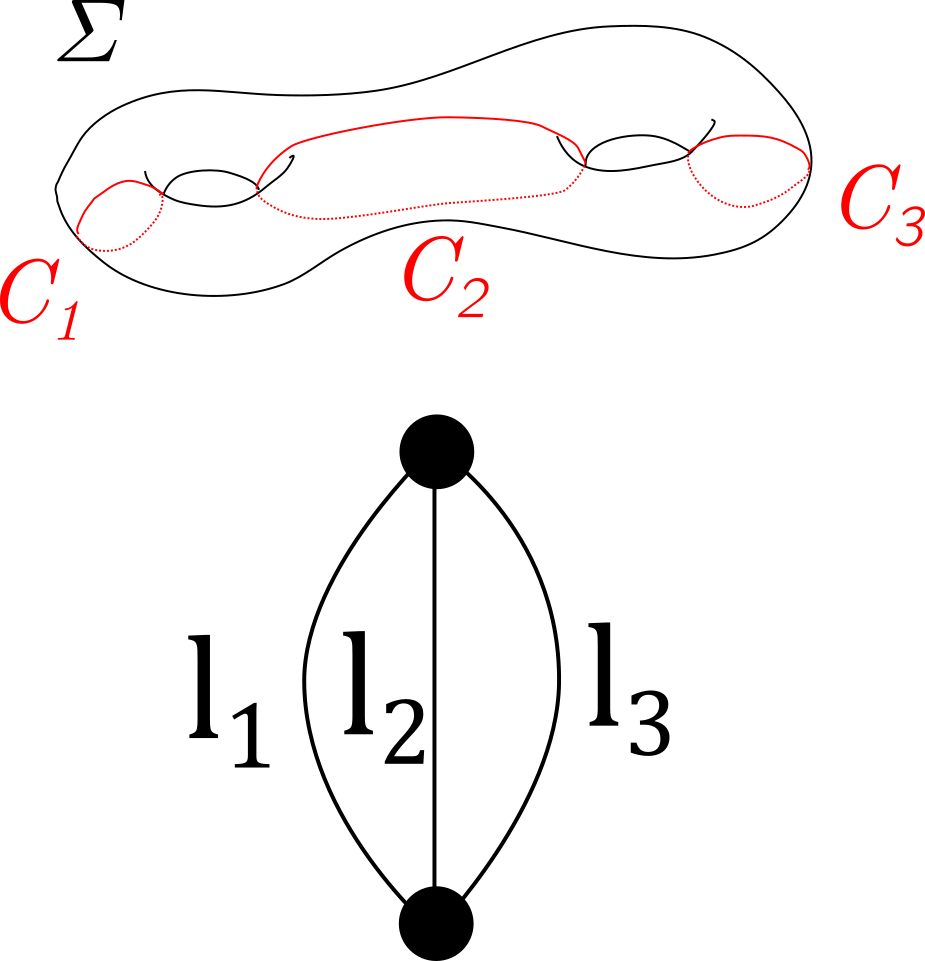
\includegraphics[width=0.4\linewidth]{g2sym_graph.png}\label{fig:sym-graph}}
		\hspace{0.1\linewidth}
		\subfloat[][The asymmetric decomposition and graph.]{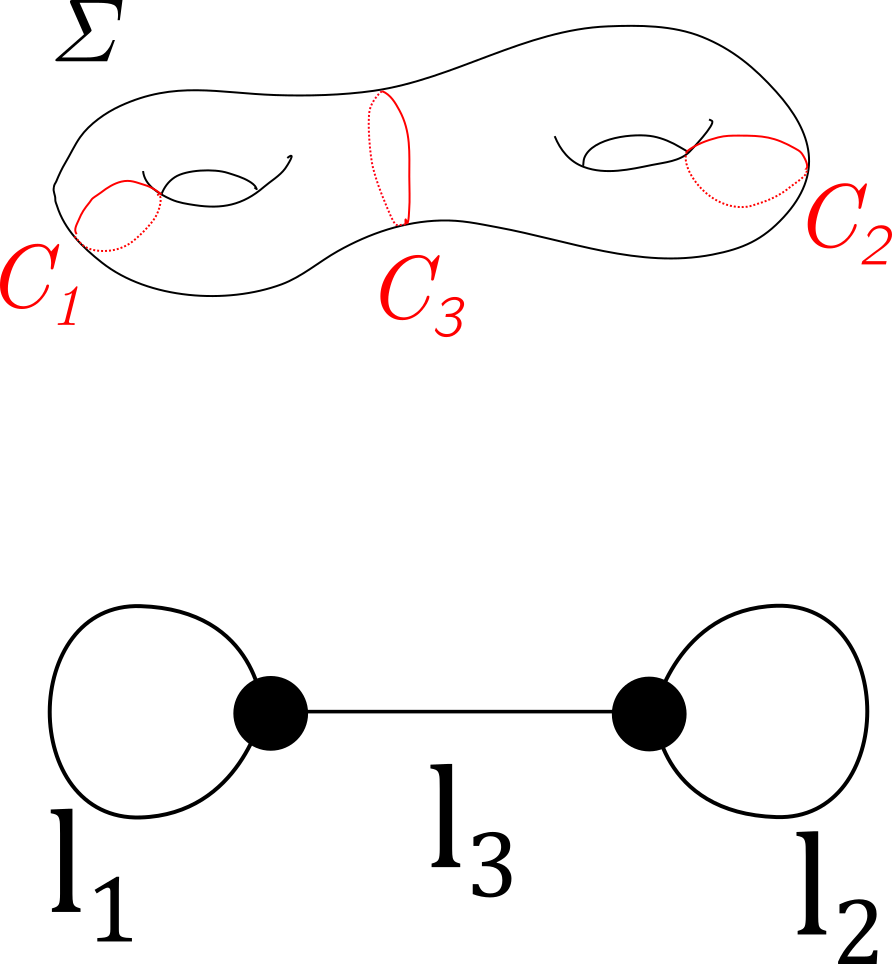
\includegraphics[width=0.4\linewidth]{g2asym_graph.png}\label{fig:asym-graph}}
		\caption{Decompositions of a genus 2 surface and the corresponding trivalent graphs.}
	\end{figure}

	\underline{Example}:
	Let $\Sigma$ be the compact Riemann surface of genus $2$, which has two trinion decompositions into two trinions. Replacing the trinions with vertices and the boundary circles with edges, we obtain the graphs in Figure \ref{fig:g2-graphs}. Let us use Theorem \ref{t:bs-count} to find the number of Bohr-Sommerfeld points for the line bundle $\LL$ over $\Sigma$ with respect to the polarisations defined by these decompositions. For the symmetric decomposition, conditions 1 and 2 are the same at each vertex, so it suffices to consider them at one vertex. Since $k=1$, each label must be either $0$ or $1$. Their sum must be even, which leaves us with four possibilities:
	\begin{equation}
		(l_1, l_2, l_3) = (0,0,0), (1,1,0), (0,1,1), \text{ or } (1,0,1).
	\end{equation}
	Finally, one can check that each of these labellings satisfies $|l_1-l_2| \leq l_3 \leq l_1+l_2$, so these are all valid labellings. Therefore Theorem \ref{t:bs-count} tells us that there are four Bohr-Sommerfeld points of $\LL$ in the polarisation defined by the symmetric decomposition of $\Sigma$.
	
	For the asymmetric decomposition, the conditions at each vertex must be checked separately, as they are different. Denoting the edges at the two vertices by $l^1_i$ and $l^2_i$, we have that
	\begin{align}
		(l^1_1,l^1_2,l^2_3) &= (l_1, l_1, l_3), & (l^2_1,l^2_2,l^2_3) &= (l_2, l_2, l_3).
	\end{align} 
	Once again since $k=1$ each label must be either $0$ or $1$. Their sum at each vertex must be even, which means $2l_1 + l_3$ and $2l_2 + l_3$ must be even. This forces $l_3$ to be zero, and we're left with the following possibilities:
	\begin{equation}
		(l_1,l_2,l_3) = (0,0,0), (1,0,0), (0,1,0), (1,1,0).
	\end{equation}
	Once again, one can check that each of these labellings satisfies $|l^i_1-l^i_2| \leq l^i_3 \leq l^i_1+l^i_2,$ ($i=1,2$) and is therefore a valid labelling of the graph. Thus Theorem \ref{t:bs-count} tells us that there are also four Bohr-Sommerfeld points of $\LL$ in the polarisation defined by the asymmetric decomposition of $\Sigma$.
	
	For higher values of $k$, a computer-assisted search finds that the number of labellings of these two graphs agree, and is equal to $10, 20, 35$ for $k=2, 3, 4$ and so on.  

	One important consequence of this theorem is that the number of Bohr-Sommerfeld points can be computed by counting points in the intersection of the period lattice $\Lambda$ with the moment polytope defined by equation \ref{e:trinion-ineqs}. In the next chapter, we will discuss the construction of another moduli space $P$ which is the toric variety corresponding to this moment polytope. From the theory of toric varieties, we know there is a line bundle over $P$ corresponding to the polytope, with a basis of sections given by the Bohr-Sommerfeld points. It will then remain to show that this line bundle over $P$ corresponds to the prequantum line bundle over $\MM$ in a way which preserves the space of sections.
	
	